
\begin{center}
Code at \url{https://github.com/cedrict/fieldstone/tree/master/python_codes/fieldstone_85}
\end{center}

\par\noindent\rule{\textwidth}{0.4pt}

{\sl This stone was developed with input from Rens Elbertsen, Bart Root, and Ross Maguire}. 
\index{contributors}{R. Elbertsen}
\index{contributors}{B. Root}
\index{contributors}{R. Maguire}

\par\noindent\rule{\textwidth}{0.4pt}
%%%%%%%%%%%%%%%%%%%%%%%%%%%%%%%%%%%%%%%%%%%%%%%%%%%%%%%%%%%%%%%%%%%%%%%%%%%%%%%%%%%%%%%%%%%%%%

\vspace{1cm}

\index{general}{S20RTS}
\index{general}{S40RTS}


The S20RTS \cite{rivw99} and S40RTS \cite{ridv11} are commonly used shear-velocity models for the mantle.
The dataset are widely available and used (in Specfem, in Aspect, ...) and come in the form of two 
files {\sl S20RTS.sph} and {\sl S40RTS.sph} (supplemented by a file with the location of the 
knots of the 21 splines used for the radial interpolation). 
Each {\sl .sph} file has a 1 line header, and the first number on this line indicates 
the maximum degree number $l$ (20 or 40, then)\footnote{
"The header lines in the sph file includes a 24 followed by 3 zeroes and 21 ones. 
This indicates that the first three splines, which apply to the crust, have been turned off."
J. Ritsema, pers. comm.}. The rest of these files consists of many rows and colums of numbers.

Let us recall that for a given value of the degree $l$ the order $m$ is such that $-l \le m \le +l$, i.e. 
there are $2l+1$ values of $m$ for a single value of $l$. Concretely:
\begin{itemize}
\item $l=0$, $m=1$ 
\item $l=1$, $m=-1,0,+1$ 
\item $l=2$, $m=-2,-1,0,+1,+2$ 
\item $l=3$, ...
\end{itemize}
The first few lines of {\sl S20RTS.sph} are shown hereunder:
\begin{tiny}
\begin{verbatim}
             20 111111111111111111111  24 000111111111111111111111 
  0.1534E-01
  0.1590E-01 -0.1336E-01  0.3469E-02
 -0.3480E-02  0.1165E-01  0.8376E-02  0.2158E-01 -0.9923E-02
 -0.1301E-02 -0.5792E-02  0.1049E-02 -0.7702E-02  0.1281E-02  0.1419E-01  0.8916E-02
  0.1353E-02 -0.5517E-02 -0.1429E-02 -0.1105E-01 -0.1247E-02  0.4788E-02 -0.8670E-03 -0.2317E-03  0.3142E-01
 -0.7365E-02 -0.1193E-01 -0.4838E-02 -0.1277E-01  0.1034E-03  0.6585E-02 -0.1351E-01  0.2126E-01 -0.1926E-01 -0.4675E-02 -0.7870E-02
  0.5379E-02  0.7332E-02  0.9048E-02 -0.7672E-02  0.1306E-01 -0.2900E-02 -0.1380E-01 -0.2366E-02  0.7911E-02 -0.9940E-02 -0.1281E-02  0.1321E-02 -0.1439E-02
\end{verbatim}
\end{tiny}

We see that the first line (after the header) contains one coefficient, corresponding to ${l=0},{m=0}$. 
The second line contains three coefficients which correspond to ${l=1},{m=-1,0,1}$ (not 
per se in that order -- see what follows). The third line contains 5 
coefficients, the fourth 7, etc ... 
In the case of S20RTS this goes on until $l=20$ and the line therefore contains 41 coefficients.
In the case of S40RTS this goes on until $l=40$ and the line contains 81 coefficients.
Unfortunately only 11 numbers are stored on a single line so the 81 coeffs corresponding 
to $l=40$ (for instance)
are spread across many lines, which makes read in the file a bit of nightmare. 
Both S20RTS and S40RTS models are composed of 21 concentric layers (from the moho down 
to the core-mantle boundary) 
so the above structure is repeated 21 times in the files. 
The structure of the file is explained in the \aspect manual (but it remains a mystery 
as to where this information comes from since it is not explained in the papers) 
in a cookbook authored by Jacqueline Austermann: \index{contributors}{J. Austermann} 
{\color{brown}
"The first number in the first line denotes the maximum degree. This is followed in
the next line by the spherical harmonic coefficients from the surface down to the
CMB. The coefficients are arranged in the following way:\\
$a_{00}$ \\
$a_{10}$ $a_{11}$ $b_{11}$ \\
$a_{20}$ $a_{21}$ $b_{21}$ $a_{22}$ $b_{22}$ \\
... \\
$a_{lm}$ is the cosine coefficient of degree $l$ and order $m$; $b_{lm}$ is
the sine coefficient of degree $l$ and order $m$."}

\begin{center}
\includegraphics[width=5cm]{python_codes/fieldstone_85/images/fun}
\end{center}


In the file {\sl aspect/source/initial\_temperature/S40RTS\_perturbation.cc} it is 
indicated that the implementation is based on Eq.~(B.99) of Dahlen \& Tromp \cite{datr98}, 
i.e. the velocity anomaly on any of the shells 
(i.e. at constant radius) at coordinate $(\theta,\phi)$ can be computed as follows:
\[
f = \sum_{l=0}^\infty \left[a_{l0} X_{l0}(\theta) + \sqrt{2} \sum_{m=1}^l X_{lm}(\theta) 
\left(a_{lm} \cos m\phi + b_{lm} \sin m\phi \right) \right]
\]
Note however that the implementation of Ritsema does {\it not} include 
the $\sqrt{2}$ term (go figure...) and this 
was the nature of a later pull request in Aspect\footnote{\url{https://github.com/geodynamics/aspect/pull/966}} 
so that the used formula is simply:
\[
\boxed{
f = \sum_{l=0}^\infty \left[a_{l0} X_{l0}(\theta) + \sum_{m=1}^l X_{lm}(\theta) 
(a_{lm} \cos m\phi + b_{lm} \sin m\phi) \right]
}
\]
with $X_{lm}(\theta)$ given by Eq.(B.58) of  \cite{datr98}:
\[
\boxed{
X_{lm} = (-1)^m \sqrt{ \frac{2l+1}{4\pi} \frac{(l-m)!}{(l+m)!} } P_l^m(\cos\theta)
}
\]
and note that in this equation $P_l^m$ does not contain the $(-1)^m$ term.

\begin{center}
\includegraphics[width=3cm]{images/sphcoord}\\
{\captionfont Spherical coordinates conventions}
\end{center}

In these equations $\theta$ is the colatitude ($0\le\theta\le \pi$ from North pole to South pole), $\phi$
is the longitude ($0\le\phi\le 2\pi$) and $P_l^m$ are associated Legendre polynomials. 
\index{general}{Legendre Polynomials}

This stone uses the {\tt scipy.special.lpmv} function for the product $(-1)^m P_l^m(x)$:
\begin{center}
\includegraphics[width=11cm]{python_codes/fieldstone_85/images/lpmv}
\end{center}

In \textcite{ridv11} (2011), one reads: "We use the same 
spline functions as in \textcite{rivw04} (2004) to parametrize vertical 
variation of shear velocity. The separation of the spline functions
increases with depth. Relatively dense spline distribution helps to
accommodate strong vertical shear-velocity variations across the
lithosphere–asthenosphere boundary and the phase transition in the
transition zone albeit at the expense of the vertical resolution at
the base of the mantle."
Unfortunately the 2004 paper does not reveal the values of the spline knots, but the values
are available in the {\sl splhsetup.f} file included in the tools available 
on J. Ritsema's website \url{https://jritsema.earth.lsa.umich.edu/Research.html}.

\begin{center}
\begin{tabular}{cccl}
\hline 
normalised & radius & depth & spline number\\
\hline 
\hline 
1.00000  & 6346619.       &  24381          &0 (moho)\\
0.96512  & 6296625.16464  &  74374.83536    &1\\
0.92675  & 6241629.079125 &  129370.920875  &2\\
0.88454  & 6181129.08513  &  189870.91487   &3\\
0.83810  & 6114566.19195  &  256433.80805   &4\\
0.78701  & 6041338.409595 &  329661.590405  &5\\
0.73081  & 5960786.415695 &  410213.584305  &6\\
0.66899  & 5872179.222405 &  498820.777595  &7\\
0.60097  & 5774685.510215 &  596314.489785  &8\\
0.52615  & 5667445.293425 &  703554.706575  &9\\
0.44384  & 5549469.58848  &  821530.41152   &10\\
0.35329  & 5419683.413255 &  951316.586745  &11\\
0.25367  & 5276897.120865 &  1094102.879135 &12\\
0.14409  & 5119835.065855 &  1251164.934145 &13\\
0.02353  & 4947035.272535 &  1423964.727465 &14\\
-0.10909 & 4756949.766645 &  1614050.233355 &15\\
-0.25499 & 4547829.910595 &  1823170.089405 &16\\
-0.41550 & 4317769.40275  &  2053230.59725  &17\\
-0.59207 & 4064689.944335 &  2306310.055665 &18\\
-0.78631 & 3786283.907055 &  2584716.092945 &19\\
-1.00000 & 3480000.       &  2891           &20  (CMB) \\
\hline
\end{tabular}\\
{\captionfont Spline knots. These range from radius 3480km (cmb) to radius 6346.619km (moho) 
as defined in Ritsema's file getfdp.f and splhsetup.f}
\end{center}

The values in the table above seem to correspond to the figure taken from 
Ritsema et al (2004) \cite{rivw04} shown hereunder: 
\begin{center}
\includegraphics[width=5cm]{python_codes/fieldstone_85/images/rivw04splines}
\includegraphics[width=10cm]{python_codes/fieldstone_85/splines/splines.pdf}\\
{\captionfont Left: Taken from Ritsema et al (2004) \cite{rivw04}.
Right: Data obtained from R. Maguire's code on github\footnote{\url{https://github.com/romaguir/sph_models}}.
We see that the splines are zero at the depths/nodes 
indicated by the tics on the x axis, and that 
they are 1 on their respective node, i.e. $B_i(d_j)=\delta_{ij}$}
\end{center}


The structure of the code is as follows: the user chooses the value of three parameters:
\begin{itemize}
\item {\codefont degree}: (maximum) degree, i.e. 20 or 40.
\item {\codefont use\_degree}: a value between 0 and {\codefont degree}
\item {\codefont depth}: depth in \si{m}.
\end{itemize}
Based on the value of {\codefont degree}, either {\filenamefont S20RTS.sph} or {\filenamefont S40RTS.sph} is read,
and the coefficients are stored in the array
\begin{verbatim}
flm = np.empty((degree+1,2*degree+1,nspline),dtype=np.float64)
\end{verbatim}
The first dimension is $l$, the second runs over $m$ (i.e. $2l+1$ values), 
and this structure is necessary for all 21 splines (third dimension).
A regular grid of $360\times 179$ longitude-latitude points is then generated (as well as their connectivity, required for vtu output). This choice is to match the default output of the Ritsema code.
Spline knots locations are then read, and converted to depths and radii between the CMB and the Moho.
A double for loop then runs over all points of the longitude-latitude plane and computes $dv/v$ as defined by the equations above 
for each spline depth, and the 21 values are then averaged/interpolated so as to return the value at the desired depth. 

The core algorithm goes as follows: we wish to compute the seismic velocity anomaly 
at location $r,\theta,\phi$.
We then compute $X_{lm}(\cos \theta)$, $\cos (m\phi)$, and $\sin (m\phi)$ 
for all the existing/relevant $(l,m)$ combinations. 
These are then combined to store the terms multiplying the $a_{lm}$ and $b_{lm}$ coefficients 
in the arrays {\codefont a\_coeffs} and {\codefont b\_coeffs}
(remember that the $(-1)^m$ term is inside the \texttt{lpmv} function).

\begin{lstlisting}
a_coeffs   = np.zeros((use_degree+1,use_degree+1), dtype=np.float64)
b_coeffs   = np.zeros((use_degree+1,use_degree+1), dtype=np.float64)
for ilat in range(0,nlat): 
    for ilon in range(0,nlon): 
        for l in range(0,use_degree+1):
            m=0
            x=np.cos(theta)
            Xlm=np.sqrt( (2*l+1)/4./np.pi ) * scipy.special.lpmv(m,l,x) 
            a_coeffs[l,0]=Xlm
            for m in range(1,l+1):
                A=math.factorial(l-m)
                B=math.factorial(l+m)
                x=np.cos(theta)
                Xlm=np.sqrt( (2*l+1)/4./np.pi*float(A)/float(B) ) * scipy.special.lpmv(m,l,x) 
                a_coeffs[l,m]=Xlm*np.cos(m*phi)
                b_coeffs[l,m]=Xlm*np.sin(m*phi)
\end{lstlisting}

For each spline shell we use the corresponding $a_{lm}$ and $b_{lm}$ coefficients to compute the 
anomaly at $(\theta,\phi)$. We end up with 21 values stored in the array {\tt shell\_values} 
which are then combined with the radial spline functions to obtain the anomaly at the desired depth:

\begin{lstlisting}
for ilat in range(0,nlat): 
    for ilon in range(0,nlon): 
        [...code snippet above...]
        shell_values=np.zeros(nspline,dtype=np.float64)  
        for ispline in range(0,nspline):
            for l in range(0,use_degree+1):
                shell_values[ispline]+=flm[l,0,ispline]*a_coeffs[l,0]
                for m in range(1,l+1):
                    alm=flm[l,2*m-1,ispline]
                    blm=flm[l,2*m,ispline]
                    shell_values[ispline]+=a_coeffs[l,m]*alm+b_coeffs[l,m]*blm
        tck=interpolate.splrep(spline_depths, shell_values)
        dv[counter]=100*interpolate.splev(depth,tck)
\end{lstlisting}

As per usual we see that the python code is ridiculously slow...


\paragraph{How to use the provided S20/S40RTS tools}:
\begin{itemize}
\item   Download {\filenamefont S20RTS\_plotting.tar.gz} at \url{https://jritsema.earth.lsa.umich.edu/Research.html}
\item   Compile everything as described in the {\filenamefont readme} file
\item   Copy the desired {\filenamefont SX0RTS.sph} file to be used in the bin directory
\item   Move to the bin directory
\item   Create a file {\filenamefont dep\_in} with on the first line the name of the .sph file (e.g. {\filenamefont S40RTS.sph}) 
        and on the second line the desired depth (in km).
\item   Run the command: {\sl ./depmaphj\_jr $<$ dep\_in $>$ dep\_out} \\
        This also creates a .raw file with 
        the same name as the .sph file chosen in {\filenamefont dep\_in}, containing the spherical harmonic coefficients 
        belonging to the chosen depth 
\item   Create a file {\filenamefont input} with the following lines (separate lines denoted by brackets):\\
        S40RTS.raw\\
        outputfile.xyz \\
        1 \\
        1 \\
        1 40\\
        -180\\ 
        where the first line is the .raw file created in the previous step, the second line is 
        the name of the output file, the third line is the step size in degrees for lon and 
        latitude centered around 0, the fourth line is a mystery to me, the fifth line 
        are the degrees that should be used and the sixth line probably has to do with the 
        starting or end point of the x-axis. 
\item   Run {\sl ./raw2xyz\_jr $<$ input} this creates a {\filenamefont file.xyz} as chosen in the input file containing lon, 
        lat and dlnvs in \%
\end{itemize}

The Ritsema code is in the {\sl S20RTS\_plotting} folder. In the {\sl bin} subfolder you will 
find my script {\filenamefont make\_map} which generates .xyz file (i.e. all the values at
the desired depth). Simply edit {\filenamefont dep\_in} and {\filenamefont input} and adjust the 
parameters.

It is worth noticing that these tools are assembled from exisiting tools and libraries (e.g. 
Numerical Recipes) and that double precision floats are not used everywhere, which, given the
thousands of summations and multiplications of terms like cosine/sine/square root/pi combined
with polynomial splines is likely 
to result in a loss of accuracy. As such, given that the values we wish to compare are around
unity one cannot hope to match the results from the python code with the fortran code with 
an accuracy better than $\sim 10^{-7}$, i.e. the accuracy of single precision floats  (and even 
that value is highly optimistic).

One can for instance select a depth which corresponds to one of the knots of the spline, 
say $d=2584716.092945\si{m}$.
In this case we know that the spline interpolation will/should not take place since the
spline associated to this depth is exactly 1 and the other ones exactly zero. 
The python and fortran codes were run at this depth and at the same resolution (nlat=179,nlon=360)
and results are found to match nicely. The {\filenamefont compare.py} script subtracts the results 
of both and generates the {\filenamefont both.ascii} file as plotted hereafter:
  

\begin{center}
\includegraphics[width=5.5cm]{python_codes/fieldstone_85/compare/both3D.png}
\includegraphics[width=5.5cm]{python_codes/fieldstone_85/compare/both2D.png}
\includegraphics[width=5.5cm]{python_codes/fieldstone_85/compare/both2Dlog.png}\\
{\captionfont Left: 3D surface plot of the signal as a function of longitude and latitude for 
both codes. Middle: same data, but projected on a 2D plane with the latitude as x-coordinate, 
with difference between both plotted in blue. Right: (absolute) difference as a function 
of latitude in log-scale.}
\end{center}

When Ritsema's code is run at this depth a file {\filenamefont dep\_out} is produced.
Its structure is not totally clear but we see that the last column corresponds to 
the weights attributed to all 21 splines. These are all nearly zero except for the 
20th which is nearly 1, as expected. This documents again the single precision character 
of the calculation since 0.999999881 is 1 at $10^{-7}$ accuracy. Rather worryingly, 
these nearby coefficients are about $10^{-7}$ and will therefore contribute to the 
synthetised  signal.  
\begin{verbatim}
 model=S20RTS.sph                                                                      
 lm=           10
 ip1+1=           1  lm-4=           6
 mfl=S20RTS
 n=            1  dep=    2584.71606    
 y1
 y2
          20           4          24          21
          20           4          24          21
 ii,dep(ii),ip,fp=            1   2584.71606               1   7.92752561E-17
 ii,dep(ii),ip,fp=            1   2584.71606               2  -4.69479181E-16
 ii,dep(ii),ip,fp=            1   2584.71606               3   1.70541370E-15
 ii,dep(ii),ip,fp=            1   2584.71606               4  -5.56919674E-15
 ii,dep(ii),ip,fp=            1   2584.71606               5   1.80295317E-14
 ii,dep(ii),ip,fp=            1   2584.71606               6  -5.83941600E-14
 ii,dep(ii),ip,fp=            1   2584.71606               7   1.89143623E-13
 ii,dep(ii),ip,fp=            1   2584.71606               8  -6.12492045E-13
 ii,dep(ii),ip,fp=            1   2584.71606               9   1.98377881E-12
 ii,dep(ii),ip,fp=            1   2584.71606              10  -6.42507532E-12
 ii,dep(ii),ip,fp=            1   2584.71606              11   2.08086742E-11
 ii,dep(ii),ip,fp=            1   2584.71606              12  -6.73884906E-11
 ii,dep(ii),ip,fp=            1   2584.71606              13   2.18269541E-10
 ii,dep(ii),ip,fp=            1   2584.71606              14  -7.06871173E-10
 ii,dep(ii),ip,fp=            1   2584.71606              15   2.28940222E-09
 ii,dep(ii),ip,fp=            1   2584.71606              16  -7.41458184E-09
 ii,dep(ii),ip,fp=            1   2584.71606              17   2.40124489E-08
 ii,dep(ii),ip,fp=            1   2584.71606              18  -7.77709275E-08
 ii,dep(ii),ip,fp=            1   2584.71606              19   2.92896800E-07
 ii,dep(ii),ip,fp=            1   2584.71606              20  0.999999881    
 ii,dep(ii),ip,fp=            1   2584.71606              21  -1.05048358E-07
\end{verbatim}

Based on these indications we can run the code and compare the obtained results 
with those obtained with Ritsema's and/or SubMachine \cite{homs18}.
Note that the data used in SubMachine are based on files (lat, lon, dvs) that 
Paula Koelemeijer provided to the lead author, 
and then interpolated between 25 km depths (pers. comm.).

\begin{center}
\includegraphics[width=12cm]{python_codes/fieldstone_85/images/ridv11}\\
{\captionfont Taken from Ritsema et al (2011) \cite{ridv11}}
\end{center}


\newpage
%......................................
\paragraph{Comparison with SubMachine - S20RTS}

\begin{center}
\includegraphics[width=5.5cm]{python_codes/fieldstone_85/images/submachine/submachine_S20RTS_25km_SMALL.jpg}
\includegraphics[width=5.5cm]{python_codes/fieldstone_85/images/submachine/submachine_S20RTS_100km_SMALL.jpg}
\includegraphics[width=5.5cm]{python_codes/fieldstone_85/images/submachine/submachine_S20RTS_600km_SMALL.jpg}\\
\includegraphics[width=5.5cm]{python_codes/fieldstone_85/images/submachine/submachine_S20RTS_1500km_SMALL.jpg}
\includegraphics[width=5.5cm]{python_codes/fieldstone_85/images/submachine/submachine_S20RTS_2800km_SMALL.jpg}
\includegraphics[width=5.5cm]{python_codes/fieldstone_85/images/submachine/submachine_S20RTS_2891km_SMALL.jpg}\\
{\captionfont Signal as obtained from SubMachine for various depths, using the Oslo colour scale, equidistant cylindrical map projection, 
16 discrete colours.}
\end{center}


\begin{center}
\includegraphics[width=5.5cm]{python_codes/fieldstone_85/images/fieldstone/fieldstone_S20RTS_25km.png}
\includegraphics[width=5.5cm]{python_codes/fieldstone_85/images/fieldstone/fieldstone_S20RTS_100km.png}
\includegraphics[width=5.5cm]{python_codes/fieldstone_85/images/fieldstone/fieldstone_S20RTS_600km.png}\\
\includegraphics[width=5.5cm]{python_codes/fieldstone_85/images/fieldstone/fieldstone_S20RTS_1500km.png}
\includegraphics[width=5.5cm]{python_codes/fieldstone_85/images/fieldstone/fieldstone_S20RTS_2800km.png}
\includegraphics[width=5.5cm]{python_codes/fieldstone_85/images/fieldstone/fieldstone_S20RTS_2891km.png}\\
{\captionfont Results obtained with Fieldstone. Coastlines and plate boundaries are obtained from Stone 69.}
\end{center}

\begin{center}
\includegraphics[width=5.5cm]{python_codes/fieldstone_85/images/fieldstone/diff_600km_S20RTS.png}\\
{\captionfont Difference between Ritsema's code results and fieldstone results at 600\si{km} depth.}
\end{center}

\newpage
%......................................
\paragraph{Comparison with SubMachine - S40RTS}

\begin{center}
\includegraphics[width=5.5cm]{python_codes/fieldstone_85/images/submachine/submachine_S40RTS_25km_SMALL.jpg}
\includegraphics[width=5.5cm]{python_codes/fieldstone_85/images/submachine/submachine_S40RTS_100km_SMALL.jpg}
\includegraphics[width=5.5cm]{python_codes/fieldstone_85/images/submachine/submachine_S40RTS_600km_SMALL.jpg}\\
\includegraphics[width=5.5cm]{python_codes/fieldstone_85/images/submachine/submachine_S40RTS_1500km_SMALL.jpg}
\includegraphics[width=5.5cm]{python_codes/fieldstone_85/images/submachine/submachine_S40RTS_2800km_SMALL.jpg}
\includegraphics[width=5.5cm]{python_codes/fieldstone_85/images/submachine/submachine_S40RTS_2891km_SMALL.jpg}\\
{\captionfont Signal as obtained from SubMachine for various depths, using the Oslo colour scale, 
equidistant cylindrical map projection, 16 discrete colours.}
\end{center}

\begin{center}
\includegraphics[width=5.5cm]{python_codes/fieldstone_85/images/fieldstone/fieldstone_S40RTS_25km.png}
\includegraphics[width=5.5cm]{python_codes/fieldstone_85/images/fieldstone/fieldstone_S40RTS_100km.png}
\includegraphics[width=5.5cm]{python_codes/fieldstone_85/images/fieldstone/fieldstone_S40RTS_600km.png}\\
\includegraphics[width=5.5cm]{python_codes/fieldstone_85/images/fieldstone/fieldstone_S40RTS_1500km.png}
\includegraphics[width=5.5cm]{python_codes/fieldstone_85/images/fieldstone/fieldstone_S40RTS_2800km.png}
\includegraphics[width=5.5cm]{python_codes/fieldstone_85/images/fieldstone/fieldstone_S40RTS_2891km.png}\\
{\captionfont Results obtained with Fieldstone. Coastlines and plate boundaries are obtained from Stone 69.}
\end{center}

\begin{center}
\includegraphics[width=5.5cm]{python_codes/fieldstone_85/images/fieldstone/diff_600km_S40RTS.png}\\
{\captionfont Difference between Ritsema's code results and fieldstone results at 600\si{km} depth.}
\end{center}

\newpage
%-------------------------------------------------------------------------
\paragraph{A look at S40RTS in \aspect} As mentioned earlier \aspect{} uses 
the same {\filenamefont SX0RTS.sph} files to arrive at $dv/v$ but it goes and extra 
step and converts this quantity first to $d\rho/\rho$ and then to a temperature 
anomaly, which is then added to a background temperature.
This is all happening in {\filenamefont /source/initial\_temperature/S40RTS\_perturbation.cc}.
In order to be able to visualise the temperature anomaly, I 
edited the \texttt{initial\_temperature} function so that it returns only the 
\texttt{temperature\_perturbation} quantity and not \texttt{background\_temperature + temperature\_perturbation}.
I then proceeded to run the {\filenamefont S20RTS.prm} cookbook with \texttt{Initial global refinement} set to 4
and looked at the temperature field which is then 
the temperature anomaly (I have also switched the Stokes and advection solvers off).

In the input file \texttt{Vs to density scaling} is set to a constant value of 0.15 while 
the \texttt{Thermal expansion coefficient} is set to 3e-5, so that $\delta T$ must be 
divided by 0.15/3e-5=5000 to obtain the original $dv/v$. This means that the 
range $[-7:7]$ for $dv/v$ becomes $[-350:350]$ for $T$:

\begin{center}
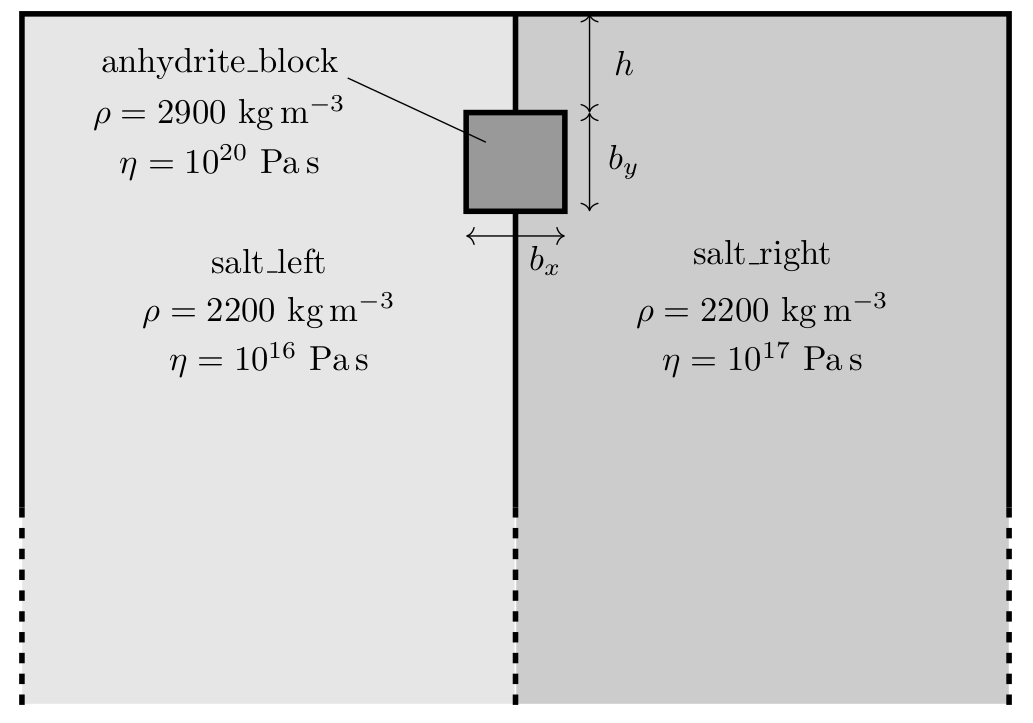
\includegraphics[width=8cm]{python_codes/fieldstone_85/aspect/aspect1}
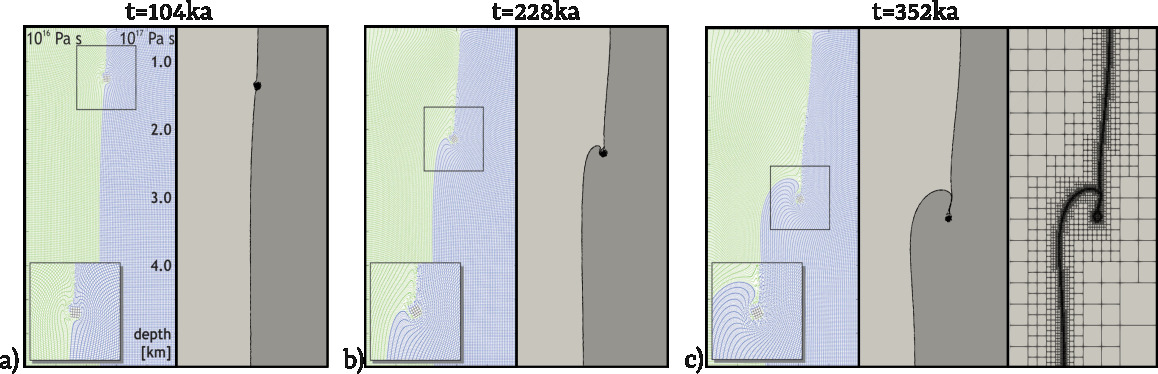
\includegraphics[width=8cm]{python_codes/fieldstone_85/aspect/aspect2}\\
\includegraphics[width=8cm]{python_codes/fieldstone_85/aspect/fieldstone1}
\includegraphics[width=8cm]{python_codes/fieldstone_85/aspect/fieldstone2}\\
{\captionfont Top row is \aspect{}, bottom row is fieldstone, depth of 100km.}
\end{center}

There is a good (but not perfect) agreement between \aspect{} and fieldstone...








